\documentclass[a4paper,11pt]{ltjsarticle}

\usepackage{amsmath,amssymb,mathtools,bm}
\usepackage{graphicx}
\usepackage{xcolor}
\usepackage[numbers,sort&compress]{natbib}
\usepackage{url}
\usepackage{booktabs}
\usepackage{hyperref}
\hypersetup{
  colorlinks=true,
  allcolors=blue!50!black,
  bookmarksnumbered=true,
  pdftitle={模擬データの計算量},
}

\graphicspath{{../docs/figures/}}
\renewcommand{\abstractname}{要旨}

\newcommand{\repourl}{https://github.com/inuverse44/retail-cosmology}
\newcommand{\code}[1]{\texttt{#1}}

\title{模擬データの計算量\\
  \large トライアルと西友の相互相関を、帰無仮説の模擬データと比べる計算}
\author{Inuverse}
\date{\today}

\begin{document}
\maketitle

\begin{abstract}
トライアルと西友の相互相関を帰無仮説の模擬データと比べる計算では、模擬データ 1 個に約 64 秒かかる。
本ノートではその計算を工程に分け、それぞれの計算量を式で表し、実測した定数を入れて時間を見積もる。
時間の 8 割は選択関数 $S_R$ を 1 点で求める計算を約 40 万回くり返すことに使われている。
人口が大都市に集中しているため、近くの点だけを調べる工夫をしても、1 回の計算は参照の点のおよそ 4 割を調べる。
そのため 1 回の計算量は参照の点の数にほぼ比例し、全体では参照の点の数の 2 乗に比例する項が残る。
選択関数を 10 km の格子ごとに一度だけ求めておけば、この計算回数は数十分の一になると見積もれる。
\end{abstract}

\tableofcontents

\section{序論}
\label{sec:intro}

本ノートは本体のノート（\code{notes/retail-cosmology.tex}）の補足である。
本体ではトライアルと西友の相互相関関数を、二社を互いに無関係に撒いた模擬データ（帰無仮説の模擬データ）の分布と比べた。
選択関数の幅を $R = 50\,\mathrm{km}$ と $100\,\mathrm{km}$ の 2 通りにし、それぞれ模擬データを 100 個作った。
模擬データ 1 個に約 64 秒かかり、6 個ずつ同時に走らせても 1 通りに 20 分以上かかった。

本ノートの問いは、この時間がどこに使われ、何に比例して増えるかである。
\ref{sec:steps} 節では模擬データ 1 個の計算を 4 つの工程に分ける。
\ref{sec:selection} 節では時間の大半を占める選択関数の計算量を式で表す。
\ref{sec:pairs} 節では対の数え上げの計算量を表す。
\ref{sec:total} 節では実測した定数を入れて全体の時間を見積もり、実測と比べる。
\ref{sec:faster} 節では計算量のオーダーを下げる方法を述べる。

\section{模擬データ 1 個の工程}
\label{sec:steps}

模擬データ 1 個の計算は次の 4 つの工程からなる。
\begin{enumerate}
  \item 偽の店を撒く。チェーンごとに、実際の店から選択関数 $S_R$ を作り、それに従って店と同じ数の点を撒く。
    人の密集地への寄り方をそろえるときは、撒く重みに人口密度の $\gamma$ 乗を掛け、$\gamma$ を決める計算もここで行う。
  \item 自己相関の対を数える。偽の店とランダムカタログの組を、距離のビンごとに数える。
  \item 選択関数つきのランダムカタログを撒く。偽の店から選択関数を作り直し、それに従って 2 万点を撒く。
    この工程の時間には撒いた点どうしの組を数える時間も入る。
  \item 相互相関の対を数える。
\end{enumerate}
工程ごとの時間を図~\ref{fig:breakdown} に示す。
選択関数を求める工程（1 と 3）が、64.3 秒のうち 53.4 秒を占める。
\begin{figure}[t]
  \centering
  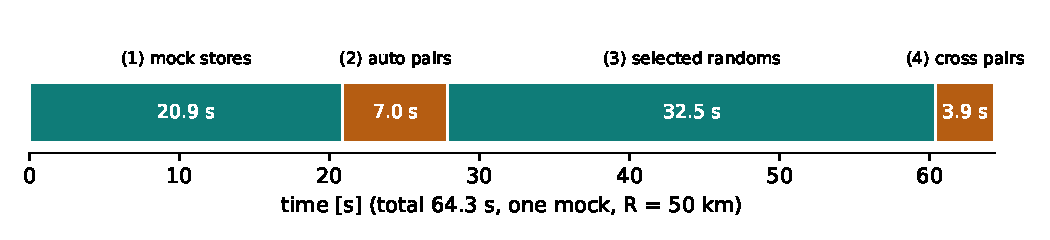
\includegraphics[width=\linewidth]{cost_breakdown.pdf}
  \caption{模擬データ 1 個（$R = 50\,\mathrm{km}$、人の密集地への寄り方もそろえる、種 1）の工程ごとの時間。
    \code{xi} の標準エラー出力の時刻（\code{data/cost/mock\_log\_R50.txt}）の差から求めた。
    緑は選択関数を求める工程、茶は対を数える工程。
    \code{scripts/plot\_cost.py} で描いた。}
  \label{fig:breakdown}
\end{figure}

記号を表~\ref{tab:symbols} にまとめる。
\begin{table}[t]
  \centering
  \caption{記号と、今回の計算での値。}
  \label{tab:symbols}
  \small
  \begin{tabular}{llr}
    \toprule
    記号 & 意味 & 値 \\
    \midrule
    $N_{\mathrm{s}}^{(a)}$ & チェーン $a$ の店の数 & 375（トライアル）、243（西友） \\
    $N_{\mathrm{p}}$ & 人口に比例して撒いた参照の点の数 & 50{,}000 \\
    $N_{\mathrm{r}}$ & ランダムカタログ 1 つの点の数 & 20{,}000 \\
    $n_{\mathrm{c}}$ & チェーンの数 & 2 \\
    $n_{\mathrm{b}}$ & 選択関数を使わない基準の数（人が住む格子、人口） & 2 \\
    $B$ & 距離のビンの数（$2$--$2000\,\mathrm{km}$ を対数で等分） & 15 \\
    $K$ & jackknife の領域の数 & 64 \\
    $R$ & 選択関数をならす幅 & $50\,\mathrm{km}$ \\
    \bottomrule
  \end{tabular}
\end{table}

\section{選択関数の計算量}
\label{sec:selection}

\subsection{1 点で求める}

選択関数は店の密度と人口の密度をそれぞれ幅 $R$ のガウス関数でならした比である（本体のノートの選択関数の式）。
\begin{equation}
  S_R(\bm{x}) = \frac{N_{\mathrm{s}}^{-1} \sum_{i} K_R(\bm{x}, \bm{x}_i)}{N_{\mathrm{p}}^{-1} \sum_{j} K_R(\bm{x}, \bm{y}_j)},
  \qquad
  K_R(\bm{x}, \bm{y}) = \exp\!\left(-\frac{c(\bm{x}, \bm{y})^2}{2\sigma_R^2}\right).
  \label{eq:selection}
\end{equation}
和は $c(\bm{x}, \bm{y}) < 3\sigma_R$ の点だけでとる。
$c$ は単位球の弦の長さ、$\sigma_R$ は大円距離 $R$ に当たる弦の長さである。

近くの点だけを拾うため、店と参照の点を、一辺 $3\sigma_R$ の立方体の格子に分けておく。
$\bm{x}$ を含む格子と、それに隣り合う格子（$3^3 = 27$ 個）にある点を調べ、そのうち $c < 3\sigma_R$ の点だけを足す（図~\ref{fig:selection}(a)）。
日本は球面の上で薄く広がっているので、実際に点があるのは平面の $3 \times 3$ 個の格子にあたる。
地図の上では、一辺がおよそ $3 \times 150 = 450\,\mathrm{km}$ の正方形の中を調べ、半径 $150\,\mathrm{km}$ の円の中を足すことになる。

$\bm{x}$ のまわりの $3 \times 3$ 個の格子に入る点の割合を $\phi_R(\bm{x})$ と書くと、1 点で求めるのにかかる時間は
\begin{equation}
  t_S(\bm{x}) \simeq t_{\mathrm{v}} \bigl(N_{\mathrm{p}} + N_{\mathrm{s}}\bigr)\, \phi_R(\bm{x})
  \label{eq:t-eval}
\end{equation}
である。$t_{\mathrm{v}}$ は 1 点を調べる時間（距離を計算し、円の中なら指数関数を足す）である。

参照の点は人口に比例して撒いてあるので、$\phi_R$ は人の多い所ほど大きい。
人口に比例して撒いた 4 万点の $\bm{x}$ で平均すると、調べた点は $19{,}427$ 点、足した点は $11{,}209$ 点だった（トライアルの選択関数、$R = 50\,\mathrm{km}$）。
$N_{\mathrm{p}} + N_{\mathrm{s}} = 50{,}375$ なので、$\langle \phi_R \rangle \simeq 0.39$ である。
近くの点だけを拾う工夫をしても、1 回の計算で参照の点の 4 割近くを調べている。
首都圏、中京圏、京阪神に人口が集まり、一辺 $450\,\mathrm{km}$ の正方形がその一つをほぼ覆うためである。
1 回の時間は $0.125\,\mathrm{ms}$ で、調べる点 1 個あたり $t_{\mathrm{v}} \simeq 6.4\,\mathrm{ns}$ になる。
西友の選択関数でも、調べた点は $19{,}452$ 点、1 回の時間は $0.124\,\mathrm{ms}$ でほぼ同じだった。

したがって、$S_R$ を 1 点で求める計算量は
\begin{equation}
  t_S = O\bigl(N_{\mathrm{p}} \langle \phi_R \rangle\bigr)
\end{equation}
である。$R$ を大きくすると $\langle \phi_R \rangle \to 1$ となり、全部の点を調べるのと同じオーダーになる。

\begin{figure}[t]
  \centering
  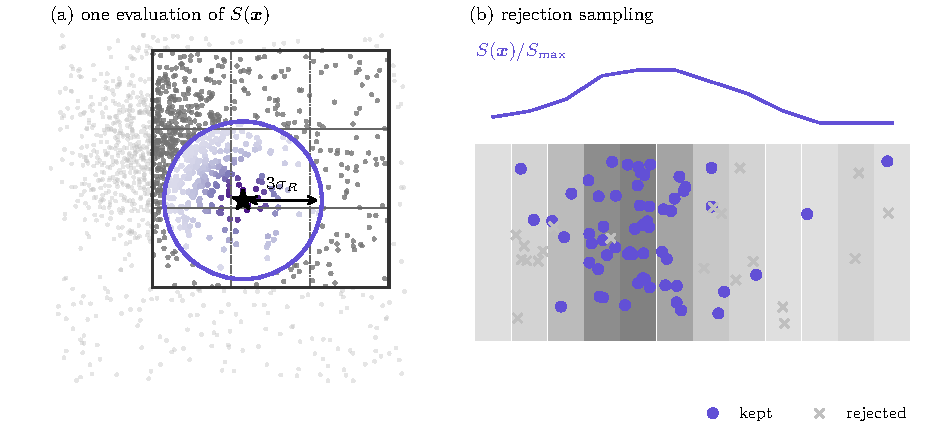
\includegraphics[width=\linewidth]{cost_selection.pdf}
  \caption{(a) $S_R(\bm{x})$ を 1 点（星印）で求める計算。灰色の点は調べない。
    青の点は $\bm{x}$ のまわりの $3 \times 3$ 個の格子（一辺 $3\sigma_R$）にあるので調べるが、円の外なので足さない。
    緑の点は円の中にあり、$\bm{x}$ に近いほど重く（濃く）足す。
    (b) 棄却法。人口に比例して候補を投げ（帯の濃さが人口）、$S_R / S_{\max}$ の確率で残す。
    残すか捨てるかを決める前に、候補ごとに $S_R$ を 1 回求める。
    どちらも模式図で、点の数は実際とは違う。}
  \label{fig:selection}
\end{figure}

\subsection{棄却法で撒く}

選択関数に従う点は棄却法で撒く（図~\ref{fig:selection}(b)）。
人口に比例して候補を投げ、確率 $S_R(\bm{x}) / S_{\max}$ で残す。
$S_{\max}$ は最初に投げた $m_0$ 個の候補での最大値である。
候補が残る割合は
\begin{equation}
  \alpha = \frac{\langle S_R \rangle_{\mathrm{pop}}}{S_{\max}}
\end{equation}
で、$\langle\cdot\rangle_{\mathrm{pop}}$ は人口で重みをつけた平均である。
$n$ 点を撒くには $n / \alpha$ 個の候補が要る。
最初の $m_0$ 個は $S_{\max}$ を決めるために必ず評価するので、$S_R$ を求める回数は
\begin{equation}
  M = \max\!\left(m_0,\ \frac{n}{\alpha}\right)
  \label{eq:candidates}
\end{equation}
である。

店が一部の地方に偏るほど、$S_{\max}$ が $\langle S_R \rangle_{\mathrm{pop}}$ より大きくなり、$\alpha$ は小さい。
実際の店から作った選択関数では、人口に比例した 4 万点で求めると、$\alpha$ はトライアルで $0.143$、西友で $0.155$ だった。
2 万点を撒くのに要る候補は $1.4 \times 10^5$ 個と $1.3 \times 10^5$ 個と見積もれる。
実際の店で走らせたときの候補は $161{,}112$ 個と $135{,}439$ 個で（\code{data/cost/real\_log\_R50.txt}）、見積もりと 15\% 程度で合う。
模擬データでは偽の店から選択関数を作るので、$\alpha$ は実際の店とは違う。
種 1 の模擬データでは、候補はトライアルで $195{,}314$ 個、西友で $45{,}850$ 個だった。

\subsection{密集地への寄り方 $\gamma$ を決める}

人の密集地への寄り方をそろえるときは、偽の店を撒く重みを $S_R(\bm{x})\, \rho(\bm{x})^{\gamma}$ にする。
$\rho$ は $\bm{x}$ を含む 1 km 格子の人口である。
$\gamma$ は、店の位置の $\ln\rho$ の平均が実際の店と等しくなるように決める。
\begin{equation}
  \frac{\sum_j S_R(\bm{y}_j)\, \rho(\bm{y}_j)^{\gamma} \ln\rho(\bm{y}_j)}{\sum_j S_R(\bm{y}_j)\, \rho(\bm{y}_j)^{\gamma}}
  = \frac{1}{N_{\mathrm{s}}} \sum_i \ln\rho(\bm{x}_i).
  \label{eq:gamma}
\end{equation}
左辺の和は参照の点 $\bm{y}_j$ についてとる。
左辺は $\gamma$ について単調に増える（$\gamma$ で微分すると重みつきの分散になる）ので、二分法で解く。

この計算ではまず $N_{\mathrm{p}}$ 個の参照の点すべてで $S_R$ を求める。
その時間は式~\eqref{eq:t-eval} から $N_{\mathrm{p}}\, t_S = O(N_{\mathrm{p}}^2 \langle\phi_R\rangle)$ で、参照の点の数の 2 乗に比例する。
二分法は 60 回で、1 回は $N_{\mathrm{p}}$ 個の指数関数を求めるだけなので、$O(60\,N_{\mathrm{p}})$ で小さい。
そのあと偽の店を棄却法で撒くとき、最初の候補は店の数の 100 倍（$m_0 = 100\,N_{\mathrm{s}}$）である。

\section{対の数え上げの計算量}
\label{sec:pairs}

対の数え上げでは2 つのカタログのすべての組について距離を計算し、ビンに入れる（図~\ref{fig:pairs}(a)）。
ビンの番号は端の並びを二分探索して求めるので、1 組は $O(\log B)$ である。
同じカタログの中の組は $N(N-1)/2$ 個、2 つのカタログの間の組は $N_1 N_2$ 個ある。
jackknife のために、組の数は領域の組 $(k, l)$ ごとに数える。
領域 $k$ を除いた数は数え直さずに足し算で求まり、その計算は $O(B K^3)$ で組の数によらない。

ビンは $2$--$2000\,\mathrm{km}$ で、日本のほとんどの組がどれかのビンに入る。
人口に比例して撒いた $5000$ 点では、$12{,}497{,}500$ 組のうち $12{,}472{,}929$ 組（$99.8\%$）がビンに入った。
近くの点だけを拾う工夫をしても、調べる組の数はほとんど減らない。
したがって、ランダムカタログどうしの組（RR）の計算量は $O(N_{\mathrm{r}}^2)$ である。

1 組の時間は領域ごとに数えるときで約 $7\,\mathrm{ns}$ だった（工程 2 の時間を組の数で割った値）。
領域を区別しない数え方では、$5000$ 点の中の組で $4.2\,\mathrm{ns}$ だった（\code{data/cost/cost\_R50.csv}）。

今の実装ではRR をチェーンごと、基準ごとに数え直している。
工程 2 ではチェーン 2 つ $\times$ 基準 2 つに、人口の点と人が住む格子の基準の組を加えて、RR を 5 回数える。
工程 3 では選択関数つきのランダムカタログごとに 1 回、計 2 回数える。
工程 4 では2 つのランダムカタログの間の組 $N_{\mathrm{r}}^2 = 4 \times 10^8$ 個を数える。

\begin{figure}[t]
  \centering
  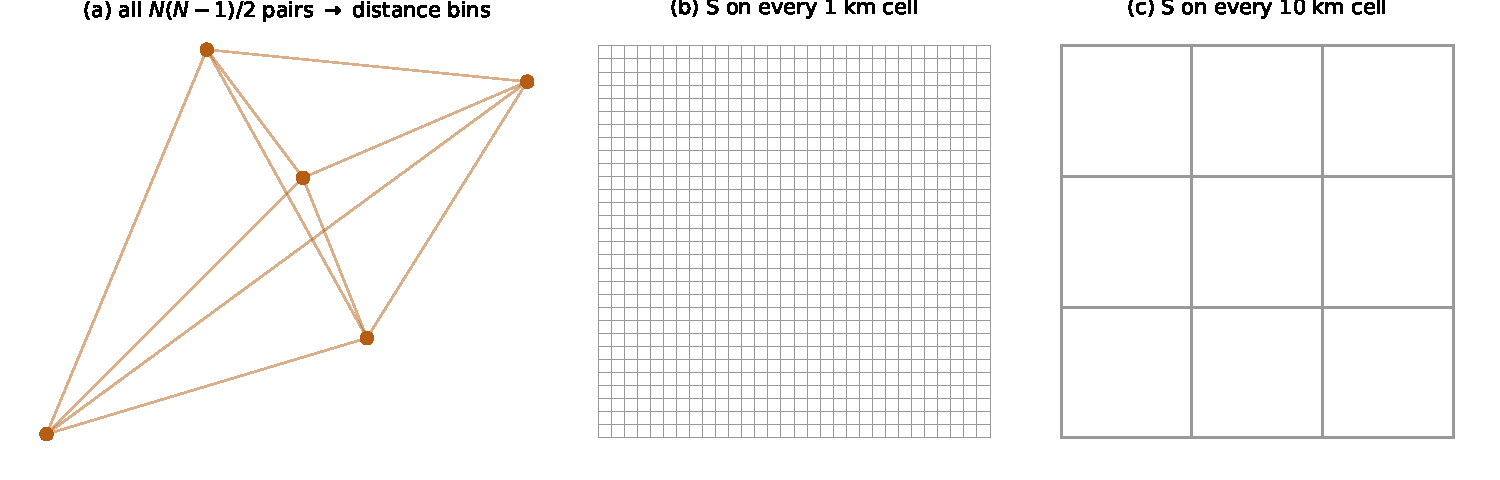
\includegraphics[width=\linewidth]{cost_pairs_grid.pdf}
  \caption{(a) 対の数え上げ。すべての組の距離を計算し、ビンに入れる。
    (b) 選択関数を 1 km 格子ごとに求める場合。日本で人が住む 1 km 格子は $176{,}964$ 個。
    (c) 10 km 格子ごとに求める場合。人が住む 10 km 格子（2 次メッシュ）は $4{,}300$ 個。
    (b) と (c) は同じ広さの範囲を描いた模式図。}
  \label{fig:pairs}
\end{figure}

\section{全体の見積もり}
\label{sec:total}

以上をまとめると、模擬データ 1 個の時間は
\begin{align}
  T \simeq{}& t_S \Bigl[\, n_{\mathrm{c}} N_{\mathrm{p}}
    + \sum_a 100\, N_{\mathrm{s}}^{(a)}
    + \sum_a \max\!\Bigl(2N_{\mathrm{r}},\ \frac{N_{\mathrm{r}}}{\alpha_a}\Bigr) \Bigr] \notag \\
  &+ t_{\mathrm{p}} \Bigl[ \bigl(n_{\mathrm{c}} n_{\mathrm{b}} + 1 + n_{\mathrm{c}}\bigr) \frac{N_{\mathrm{r}}^2}{2} + N_{\mathrm{r}}^2 \Bigr]
  \label{eq:total}
\end{align}
と書ける。
1 行目の 3 つの項は$\gamma$ を決める計算、偽の店を撒く計算、選択関数つきのランダムカタログを撒く計算である。
2 行目は RR の数え上げで、DD と DR はこれより桁違いに少ないので省いた。
オーダーで書くと
\begin{equation}
  T = O\bigl(N_{\mathrm{p}}^2 \langle\phi_R\rangle\bigr)
    + O\!\left(\frac{N_{\mathrm{r}}}{\alpha}\, N_{\mathrm{p}} \langle\phi_R\rangle\right)
    + O\bigl(N_{\mathrm{r}}^2\bigr)
\end{equation}
である。

実測した値を入れて、表~\ref{tab:estimate} で実測の時間と比べる。
$S_R$ を求める回数は、工程 1 が $2 \times 50{,}000 + 100 \times (375 + 243) = 161{,}800$ 回、工程 3 が $195{,}314 + 45{,}850 = 241{,}164$ 回である。
これに $t_S = 0.125\,\mathrm{ms}$ を掛けると、20.2 秒と 30.1 秒になる。
RR は工程 2 で $5 \times 2 \times 10^8 = 10^9$ 組、工程 3 で $4 \times 10^8$ 組、工程 4 で $4 \times 10^8$ 組である。
\begin{table}[t]
  \centering
  \caption{模擬データ 1 個の時間の見積もりと実測（$R = 50\,\mathrm{km}$、種 1）。
    見積もりは $t_S = 0.125\,\mathrm{ms}$、$t_{\mathrm{p}} = 7\,\mathrm{ns}$ として求めた。}
  \label{tab:estimate}
  \small
  \begin{tabular}{lrrrr}
    \toprule
    工程 & $S_R$ を求める回数 & RR の組 & 見積もり [s] & 実測 [s] \\
    \midrule
    1 偽の店を撒く & $161{,}800$ & --- & 20.2 & 20.9 \\
    2 自己相関の対 & --- & $1.0 \times 10^9$ & 7.0 & 7.0 \\
    3 ランダムカタログを撒く & $241{,}164$ & $4 \times 10^8$ & 32.9 & 32.5 \\
    4 相互相関の対 & --- & $4 \times 10^8$ & 2.8 & 3.9 \\
    \midrule
    計 & $402{,}964$ & $1.8 \times 10^9$ & 62.9 & 64.3 \\
    \bottomrule
  \end{tabular}
\end{table}
工程 2 の $t_{\mathrm{p}}$ は工程 2 の実測から決めたので、その行は一致して当然である。
ほかの工程は独立な見積もりで、実測と 1 秒程度で合う。
工程 4 は見積もりより 1 秒長い。2 つのカタログの間の組の数え方は、組あたりの時間が工程 2 より長いことになるが、その理由は調べていない。

時間の $83\%$（53.4 秒）は $S_R$ を求める工程にある。
$S_R$ を求める回数の $40\%$ は $\gamma$ を決める計算と偽の店の最初の候補、$60\%$ はランダムカタログの候補である。

\section{計算量を下げる方法}
\label{sec:faster}

\subsection{選択関数を粗い格子で求めておく}

$S_R$ は幅 $R = 50\,\mathrm{km}$ でならした関数なので、それより十分小さい範囲ではほとんど変わらない。
そこで、人が住む 10 km 格子（2 次メッシュ、$N_{10} = 4{,}300$ 個）の中心で $S_R$ を一度だけ求め、候補の点ではその格子の値を引くことにする（図~\ref{fig:pairs}(c)）。
$S_R$ を求める回数はチェーンごとに $M$ から $N_{10}$ に変わる。
\begin{equation}
  O\!\left(\frac{N_{\mathrm{r}}}{\alpha}\, N_{\mathrm{p}} \langle\phi_R\rangle\right)
  \ \longrightarrow\
  O\bigl(N_{10}\, N_{\mathrm{p}} \langle\phi_R\rangle\bigr) + O\!\left(\frac{N_{\mathrm{r}}}{\alpha}\right).
\end{equation}
後ろの項は格子の値を引くだけで、$S_R$ の計算に比べて無視できる。
$\gamma$ を決める計算と偽の店の候補も、同じ表から値を引ける。
すると $S_R$ を求める回数は二社で $8{,}600$ 回になり、時間は約 1 秒と見積もれる。
今の $403{,}000$ 回の約 47 分の 1 である。

ただし、格子の中で $S_R$ を一定とみなすので、値がずれる。
ずれの大きさは格子の大きさ（約 10 km）と $S_R$ の傾きの積の程度で、店の分布が急に変わる所で大きくなる。
本体の結果が変わらないことを、今の方法と比べて確かめる必要がある。

なお、1 km 格子ごとに求めておく方法では速くならない。
人が住む 1 km 格子は $176{,}964$ 個で、トライアルのランダムカタログの候補の数（$1.6$--$2.0 \times 10^5$）と同じ程度だからである。

\subsection{ならす計算を畳み込みで行う}

式~\eqref{eq:selection} の分子と分母は、点の分布とガウス関数の畳み込みである。
店と参照の点を格子に数え入れ、高速フーリエ変換で畳み込めば、すべての格子の値が $O(L \log L)$ で求まる。
$L$ は格子の数である。
この方法なら、$N_{\mathrm{p}}$ を増やしても計算量はほとんど増えない。
ただし、球面を平面の格子に写すときのゆがみを扱う必要がある。

\subsection{同じ RR を数え直さない}

人が住む格子と人口の基準のランダムカタログは、乱数の種を固定しているので、100 個の模擬データで同じである。
その RR は一度数えればよく、工程 2 の大半（約 7 秒）が 2 個目以降は要らなくなる。
1 個の模擬データの中でも、チェーンごとに同じ RR を数え直している。

\subsection{見積もり}

選択関数を 10 km 格子で求め、同じ RR を数え直さないようにすると、式~\eqref{eq:total} の残りは、工程 3 と 4 の RR（約 6 秒）と、$S_R$ の表（約 1 秒）になる。
模擬データ 1 個は 64 秒から 10 秒程度になると見積もれる。
これは式からの見積もりで、まだ実装して測ってはいない。

\section{結論}
\label{sec:conclusion}

模擬データ 1 個の時間の $83\%$ は選択関数 $S_R$ を 1 点で求める計算を約 40 万回くり返すことに使われている。
人口が大都市に集中しているため、近くの点だけを調べる工夫をしても、1 回の計算は参照の点の約 4 割を調べる。
そのため $\gamma$ を決める計算は参照の点の数の 2 乗に比例し、ランダムカタログを撒く計算は候補の数と参照の点の数の積に比例する。
選択関数を 10 km 格子で一度だけ求めれば、$S_R$ を求める回数は約 47 分の 1 になる。
対の数え上げは $O(N_{\mathrm{r}}^2)$ で、ビンが国全体の距離を覆うので、組の数は減らせない。
ただし、模擬データの間で変わらない RR は一度数えれば足りる。

\appendix

\section{再現の手順}
\label{app:reproduce}

本ノートの数字と図は、次のコマンドで作った。
\begin{verbatim}
S=data/trial_site/trial_site_clean_2026-11-03.csv,\
data/seiyu_site/seiyu_site_clean_2026-11-04.csv
target/release/xi 2026-11-03 --country jp --stores $S \
  --cross TRIAL,SEIYU --footprint 50 --mock 50:1 \
  --mock-density on --tag costlog 2> data/cost/mock_log_R50.txt
target/release/xi 2026-11-03 --country jp --stores $S \
  --cross TRIAL,SEIYU --footprint 50 \
  --tag costreal 2> data/cost/real_log_R50.txt
cargo run --release --bin cost -- 50 40000
uv run scripts/plot_cost.py
\end{verbatim}
時間は Apple M1 の Mac で、1 つのスレッドで測った（ほかの計算を止めた状態）。
別の計算機では $t_{\mathrm{v}}$ と $t_{\mathrm{p}}$ が変わるが、回数と組の数は変わらない。

\end{document}
